\section{Results}
\label{sec:res}
\begin{figure}[h]
	\centering
	\captionsetup{justification=centering}
	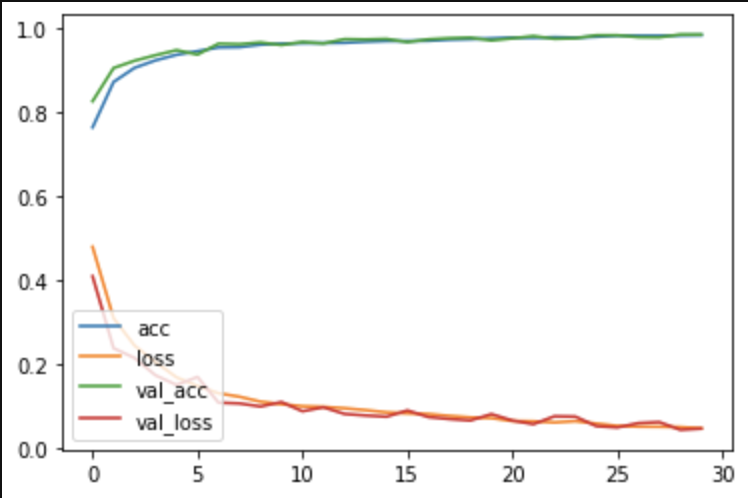
\includegraphics[width=0.4\columnwidth]{Figures/CNNMetrics.png}
	\caption{Training and validation metrics for the CNN model}
	\label{fig:cnnmetrics}
\end{figure}

We can see from the results illustrated in Figure~\ref{fig:cnnmetrics} that the CNN model is very promising, with a validation accuracy of 98.5\% over 30 epochs of training we can conclude that the a CNN is suitable for classifying the morphology of galaxies. With more training data and optimization of the model architecture and hypertuning the parameters the accuracy can be very well increased to over 99\%.